\documentclass[12pt, leqno]{article} %% use to set typesize
\include{common}

\begin{document}

\hdr{2019-10-02}

\section{Cricket chirps: an example}

Did you know that you can estimate the temperature by listening to the
rate of chirps?  The data set in Table~\ref{table1}%
\footnote{Data set originally attributed to
  \url{http://mste.illinois.edu}}.  represents measurements of the
number of chirps (over 15 seconds) of a striped ground cricket at
different temperatures measured in degrees Farenheit.  A plot
(Figure~\ref{fig2}) shows that the two are roughly correlated: the
higher the temperature, the faster the crickets chirp.  We can
quantify this by attempting to fit a linear model
\[
  \mbox{temperature} = \alpha \cdot \mbox{chirps} + \mbox{beta} + \epsilon
\]
where $\epsilon$ is an error term.  To solve this problem by linear
regression, we minimize the Euclidean norm of the residual
\[
  r = b-Ax
\]
where
\begin{align*}
  b_{i} &= \mbox{temperature in experiment } i \\
  A_{i1} &= \mbox{chirps in experiment } i \\
  A_{i2} &= 1 \\
  x &= \begin{bmatrix} \alpha \\ \beta \end{bmatrix}
\end{align*}
MATLAB and Octave are capable of solving least squares problems using
the backslash operator; that is, if {\tt chirps} and {\tt temp} are
column vectors in MATLAB, we can solve this regression problem as
\begin{lstlisting}
  A = [chirps, ones(ndata,1)];
  x = A\temp;
\end{lstlisting}
The algorithms underlying that backslash operation will make up
most of the next lecture.

\begin{figure}
  \begin{center}
    \begin{tikzpicture}
      \begin{axis}[xlabel={Chirps},ylabel={Degrees},grid=major]
        \addplot[only marks] table {data/cricket.dat};
        \addplot table[x=chirp,y=fit]{data/cricket.dat};
      \end{axis}
    \end{tikzpicture}
  \end{center}
  \caption{Cricket chirps vs.~temperature and a model fit via
    linear regression.}
  \label{fig2}
\end{figure}

\begin{table}
  \small
  \begin{tabular}{l|cccccccccccccccccc}
    Chirp &
    20& 16& 20& 18& 17& 16& 15& 17& 15& 16& 15& 17& 16& 17& 14 \\
    Temp &
    89& 72& 93& 84& 81& 75& 70& 82& 69& 83& 80& 83& 81& 84& 76
  \end{tabular}
  \caption{Cricket data: Chirp count over a 15 second period vs.~temperature
    in degrees Farenheit.}
  \label{table1}
\end{table}

In more complex examples, we want to fit a model involving more than
two variables.  This still leads to a linear least squares problem,
but one in which $A$ may have more than one or two columns.  As we
will see later in the semester, we also use linear least squares
problems as a building block for more complex fitting procedures,
including fitting nonlinear models and models with more complicated
objective functions.

\section{The least squares problem}

The ordinary linear least squares problem, simply stated, is
\[
  \operatorname{minimize}_x \|Ax-b\|_2^2
\]
where $A \in \bbR^{m \times n}$ with $m > n$.
Unless otherwise stated, we will assume that undecorated norms
refer to the two-norm for this part of the course.

\subsection{The normal equations}

\begin{figure}
  \begin{center}
  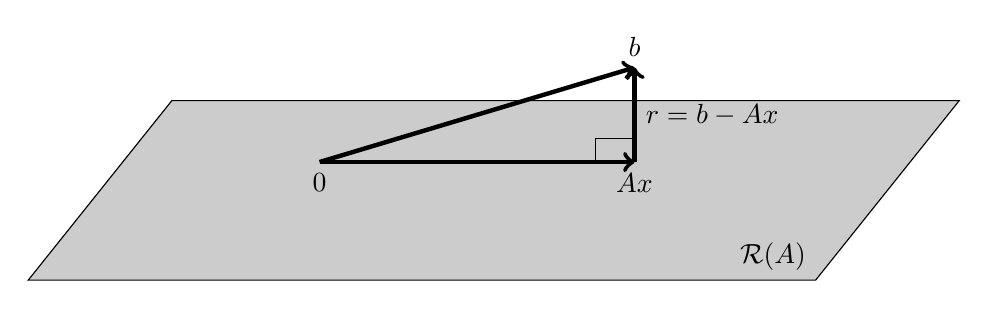
\begin{tikzpicture}
    \begin{scope}[xslant=0.8,xscale=5,yscale=3]
      \draw[fill=black!20] (-0.5,-0.5) rectangle (1.5,0.26);
      \draw[ultra thick,->]
        (0,0) node[below] {$0$} --
        (0.8,0) node[below] {$Ax$};
      \node[above left] at (1.5,-0.5) {$\mathcal{R}(A)$};
    \end{scope}
    \begin{scope}[xscale=5,yscale=3]
    \draw[ultra thick,->]
      (0,0) -- (0.8,0.4) node[above] {$b$};
    \draw[ultra thick,->]
      (0.8,0) -- (0.8,0.4) node[midway,right] {$r=b-Ax$};
    \draw (0.7,0) -- (0.7,0.1) -- (0.8,0.1);
    \end{scope}
  \end{tikzpicture}
  \end{center}
  \caption{Picture of a linear least squares problem.  The vector $Ax$
           is the closest vector in $\mathcal{R}(A)$ to a target
           vector $b$ in the Euclidean norm.  Consequently, the
           residual $r = b-Ax$ is normal (orthogonal) to
           $\mathcal{R}(A)$.}
  \label{fig1}
\end{figure}

The quantity
$r = Ax-b$ is the least squares residual; unlike in the case of
linear systems, this residual is not generally zero at the exact
minimizer.  We may write $\|r\|^2$ as a quadratic function of $x$,
\[
  \|r\|^2 = x^T A^T A x - 2 x^T A^T b + b^T b,
\]
and taking variations with respect to $x$ gives
\[
  \delta (\|r\|^2) = 2 \delta x^T (A^T A x - A^T b) = 2 \delta x^T A^T r.
\]
Thus, at a minimizer, we require $A^T r = 0$.  Geometrically, this says
that at the minimizer, $r$ is orthogonal to (normal to) any vector
in the range space of $A$ (see Figure~\ref{fig1}); hence, we call this the {\em normal equations}.

\subsection{The Moore-Penrose pseudoinverse}

If $A$ is full rank, then $A^T A$ is symmetric and positive definite,
and we have that
\[
  x = (A^T A)^{-1} A^T b \equiv A^\dagger b
\]
is a linear function of the right hand side $b$.  We call $A^\dagger$
the {\em Moore-Penrose pseudoinverse} of $A$.  It is a pseudoinverse
because $A^\dagger A = I$; this implies as well that $P = A A^\dagger$
is a projector (i.e.~$P^2 = P$).  For the purposes of this class, we
will call this ``the pseudoinverse,'' but though the Moore-Penrose
pseudoinverse is the most common and well-known, it is useful to know
that it is not the {\em only} pseudoinverse out there -- the Drazin
pseudoinverse is a good alternate example.


\section{Why least squares?}

Why is the ordinary least squares problem interesting?
There are at least three natural responses.

\begin{enumerate}
  \item {\bf Simplicity:}
  The least squares problem is one of the simplest formulations
  around for fitting linear models.  The quadratic loss model
  is easy to work with analytically; it is smooth; and it leads
  to a problem whose solution is linear in the observation data.

  \item {\bf Statistics:}
  The least squares problem is the optimal approach to parameter
  estimation among linear unbiased estimators, assuming independent
  Gaussian noise.  The least squares problem is also the maximum likelihood
  estimator under these same hypotheses.

  \item {\bf It's a building block:}
  Linear least squares are not the right formulation for all regression
  problems --- for example, they tend to lack robustness in the face of
  heavy-tailed, non-Gaussian random errors.  But even for these cases,
  ordinary least squares is a useful {\em building block}.
  Because least squares problems are linear in the observation vector,
  they are amenable to direct attack by linear algebra methods in a way
  that other estimation methods are not.  The tools we
  have available for more complex fitting boil down to linear algebra
  subproblems at the end of the day, so it is useful to learn how to work
  effectively with linear least squares.
\end{enumerate}

\section{Least squares and statistical models}

Consider the model
\[
  y_i = \sum_{j=1}^n c_j x_{ij} + \epsilon_i
\]
where the {\em factors} $x_{ij}$ for example $j$ are known,
and the observations $y_i$ are assumed to be an (unknown)
combination of the factor values plus a small independent
Gaussian noise term $\epsilon_i \tilde N(0,\sigma^2)$.
In terms of a linear system, we have
\[
  y = X c + \epsilon.
\]
A {\em linear unbiased estimator} for $c$ is a linear combination
of the observations whose expected value is $c$; that is, we
need a matrix $M \in \bbR^{n \times m}$ such that
\[
  E[M^T y] = M^T X c = c.
\]
That is, $M$ should be a pseudo-inverse of $X$.

According to the Gauss-Markov theorem, the choice $M = X^\dagger$
is optimal, and the estimator $\hat{c} = X^\dagger y$
is the {\em best linear unbiased estimator} (BLUE).  That is,
it is the linear unbiased estimator of $c$ such that for any
$u \in \bbR^n$,  $u^T \hat{c}$ has the smallest variance possible.
Alternately (and equivalently),
$\operatorname{Var}(\hat{c}) \succeq \operatorname{Var}(\tilde{c})$
for any linear unbiased estimator $\tilde{c}$.  Here $\succeq$ refers
to the partial ordering among symmetric matrices: if $A$ and $B$
are symmetric matrices, then
\[
  A \succeq B \quad \equiv \quad (A-B) \mbox{ is positive semidefinite}.
\]

What if we have more interesting noise?  For example, what if the
noise variables $\epsilon$ are drawn from a multivariate Gaussian
distribution with mean zero and positive definite covariance matrix $C$?
In this case, it turns out that if $C = R^T R$ is the
Cholesky factorization, then
\[
  z = R^{-T} \hat{\epsilon}
\]
has independent standard normal entries, and so we can apply
the Gauss-Markov theorem to the equation
\[
  R^{-T} y = R^{-T} X c + R^{-T} \epsilon.
\]
The solution $\hat{c} = (R^{-T} X)^{\dagger} R^{-T} y$ can be also
written as
\[
  \hat{c} = \operatorname{argmin}_c \|Xc-y\|^2_{C^{-1}}
\]
where
\[
  \|u\|_{C^-1}^2 \equiv u^T (C^{-1}) u.
\]
This is a generalized least squares problem; the most common version
is the weighted least squares case where the noise is assumed to
be independent, but does not have the same variance for every equation.

\section{A family of factorizations}

\subsection{Cholesky}

If $A$ is full rank, then $A^T A$ is symmetric and positive definite
matrix, and we can compute a Cholesky factorization of $A^T A$:
\[
  A^T A = R^T R.
\]
The solution to the least squares problem is then
\[
  x = (A^T A)^{-1} A^T b = R^{-1} R^{-T} A^T b,
\]
or, in MATLAB world
\begin{lstlisting}
  R = chol(A'*A, 'upper');
  x = R\(R'\(A'*b));
\end{lstlisting}

\subsection{Economy QR}

The Cholesky factor $R$ appears in a different setting as well.
Let us write $A = QR$ where $Q = AR^{-1}$; then
\[
  Q^T Q = R^{-T} A^T A R^{-1} = R^{-T} R^T R R^{-1} = I.
\]
That is, $Q$ is a matrix with orthonormal columns.  This
``economy QR factorization'' can be computed in several different
ways, including one that you have seen before in a different guise
(the Gram-Schmidt process).  MATLAB provides a numerically stable
method to compute the QR factorization via
\begin{lstlisting}
  [Q,R] = qr(A,0);
\end{lstlisting}
and we can use the QR factorization directly to solve the least
squares problem without forming $A^T A$ by
\begin{lstlisting}
  [Q,R] = qr(A,0);
  x = R\(Q'*b);
\end{lstlisting}

\subsection{Full QR}

There is an alternate ``full'' QR decomposition where we write
\[
A = QR, \mbox{ where }
Q = \begin{bmatrix} Q_1 & Q_2 \end{bmatrix} \in \bbR^{n \times n},
R = \begin{bmatrix} R_{1} \\ 0 \end{bmatrix} \in \bbR^{m \times n}.
\]
To see how this connects to the least squares problem, recall
that the Euclidean norm is invariant under orthogonal transformations,
so
\[
  \|r\|^2 = \|Q^T r\|^2 = \left\| \begin{bmatrix} Q_1^T b \\ Q_2^T
    b \end{bmatrix} - \begin{bmatrix} R_1 \\ 0 \end{bmatrix} x
  \right\|^2 = \|Q_1^T b-R_1x\|^2 + \|Q_2^T b\|^2.
\]
We can set $\|Q_1^T v-R_1 x\|^2$ to zero by
setting $x = R_1^{-1} Q_1^T b$; the result is
$\|r\|^2 = \|Q_2^T b\|^2$.

\subsection{SVD}

The full QR decomposition is useful because orthogonal transformations
do not change lengths.  Hence, the QR factorization lets us change
to a coordinate system where the problem is simple without changing
the problem in any fundamental way.  The same is true of the SVD,
which we write as
\begin{align*}
A &=
\begin{bmatrix} U_1 & U_2 \end{bmatrix}
\begin{bmatrix} \Sigma \\ 0 \end{bmatrix}
V^T & & \mbox{Full SVD} \\
&= U_1 \Sigma V^T & & \mbox{Economy SVD}.
\end{align*}
As with the QR factorization, we can apply an orthogonal
transformation involving the factor $U$ that makes the
least squares residual norm simple:
\[
\|U^T r\|^2 =
\left\| \begin{bmatrix} U_1^T b \\ U_2^T b \end{bmatrix} -
\begin{bmatrix} \Sigma V^T \\ 0 \end{bmatrix} x
\right\| =
\|U_1^T b - \Sigma V^T x\|^2 + \|U_2^T b\|^2,
\]
and we can minimize by setting $x = V \Sigma^{-1} U_1^T b$.

\end{document}
